% ======== Slide 1 =========
\begin{frame}
\frametitle{Цель и задачи}
	\textbf{Актуальность (опционально)} ....
	
	\textbf{Цель работы --} ..... 
	
	\textbf{Задачи:} ..... 
	
   	\begin{itemize}
   		\item ...
   		\item ...
   		\item ...
   	\end{itemize}
\end{frame}


% ======== Slide 2 =========

\begin{frame}
\frametitle{Название слайда}
Пример многоуровневого списка

\begin{enumerate}
  \item \textbf{Задача 1}
  \begin{itemize}
    \item Подзадача 1-1
    \item Подзадача 1-2
  \end{itemize}
  \item \textbf{Задача 2}
  \begin{itemize}
    \item Подзадача 2-1
    \item Подзадача 2-2
    \item Подзадача 2-3
  \end{itemize}
  \item \textbf{Задача 3}
  \begin{itemize}
    \item Подзадача 3-1
    \item Подзадача 3-2
    \item Подзадача 3-3
  \end{itemize}
\end{enumerate}
\end{frame}

% ======== Slide 3 =========

\begin{frame}
\frametitle{Название слайда}
Пример размещения текста и нескольких рисунков
	\begin{center}
	\begin{minipage}[h]{0.39\linewidth}
		\begin{center}
			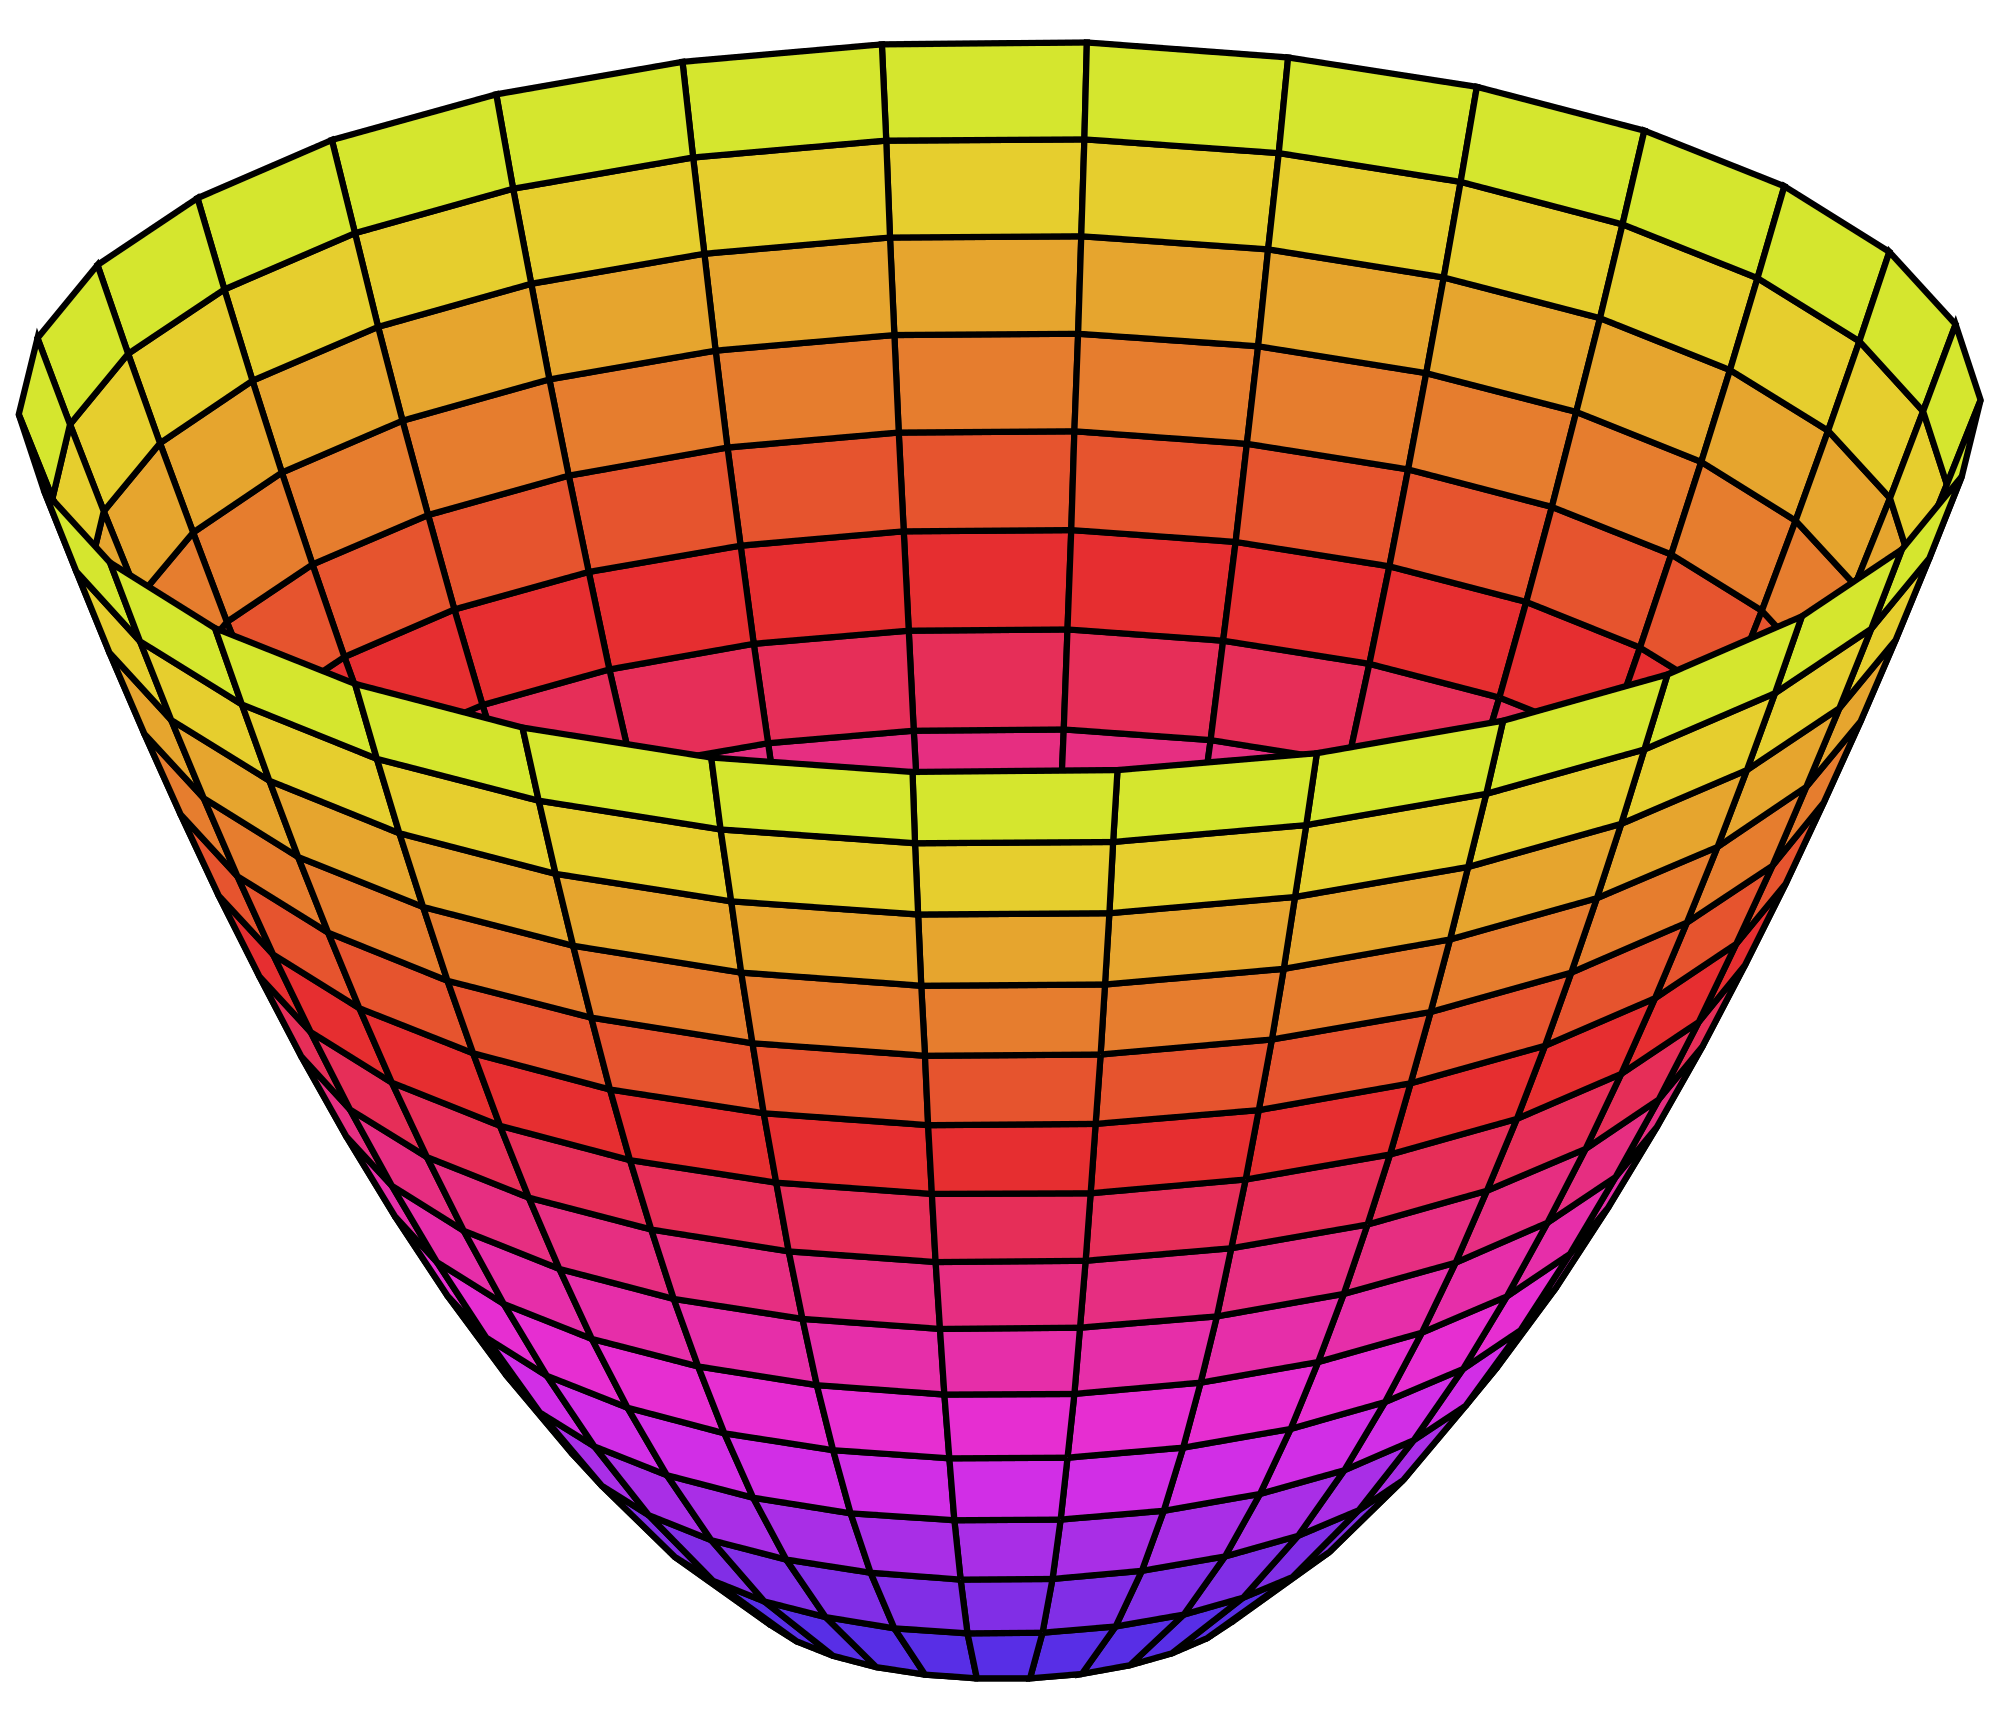
\includegraphics[scale=0.065]{paraboloid.png}
			
			\small Рисунок 1 --- Параболоид	
		\end{center}
	\end{minipage}
	\hfill 
	\begin{minipage}[h]{0.59\linewidth}
		\begin{center}
			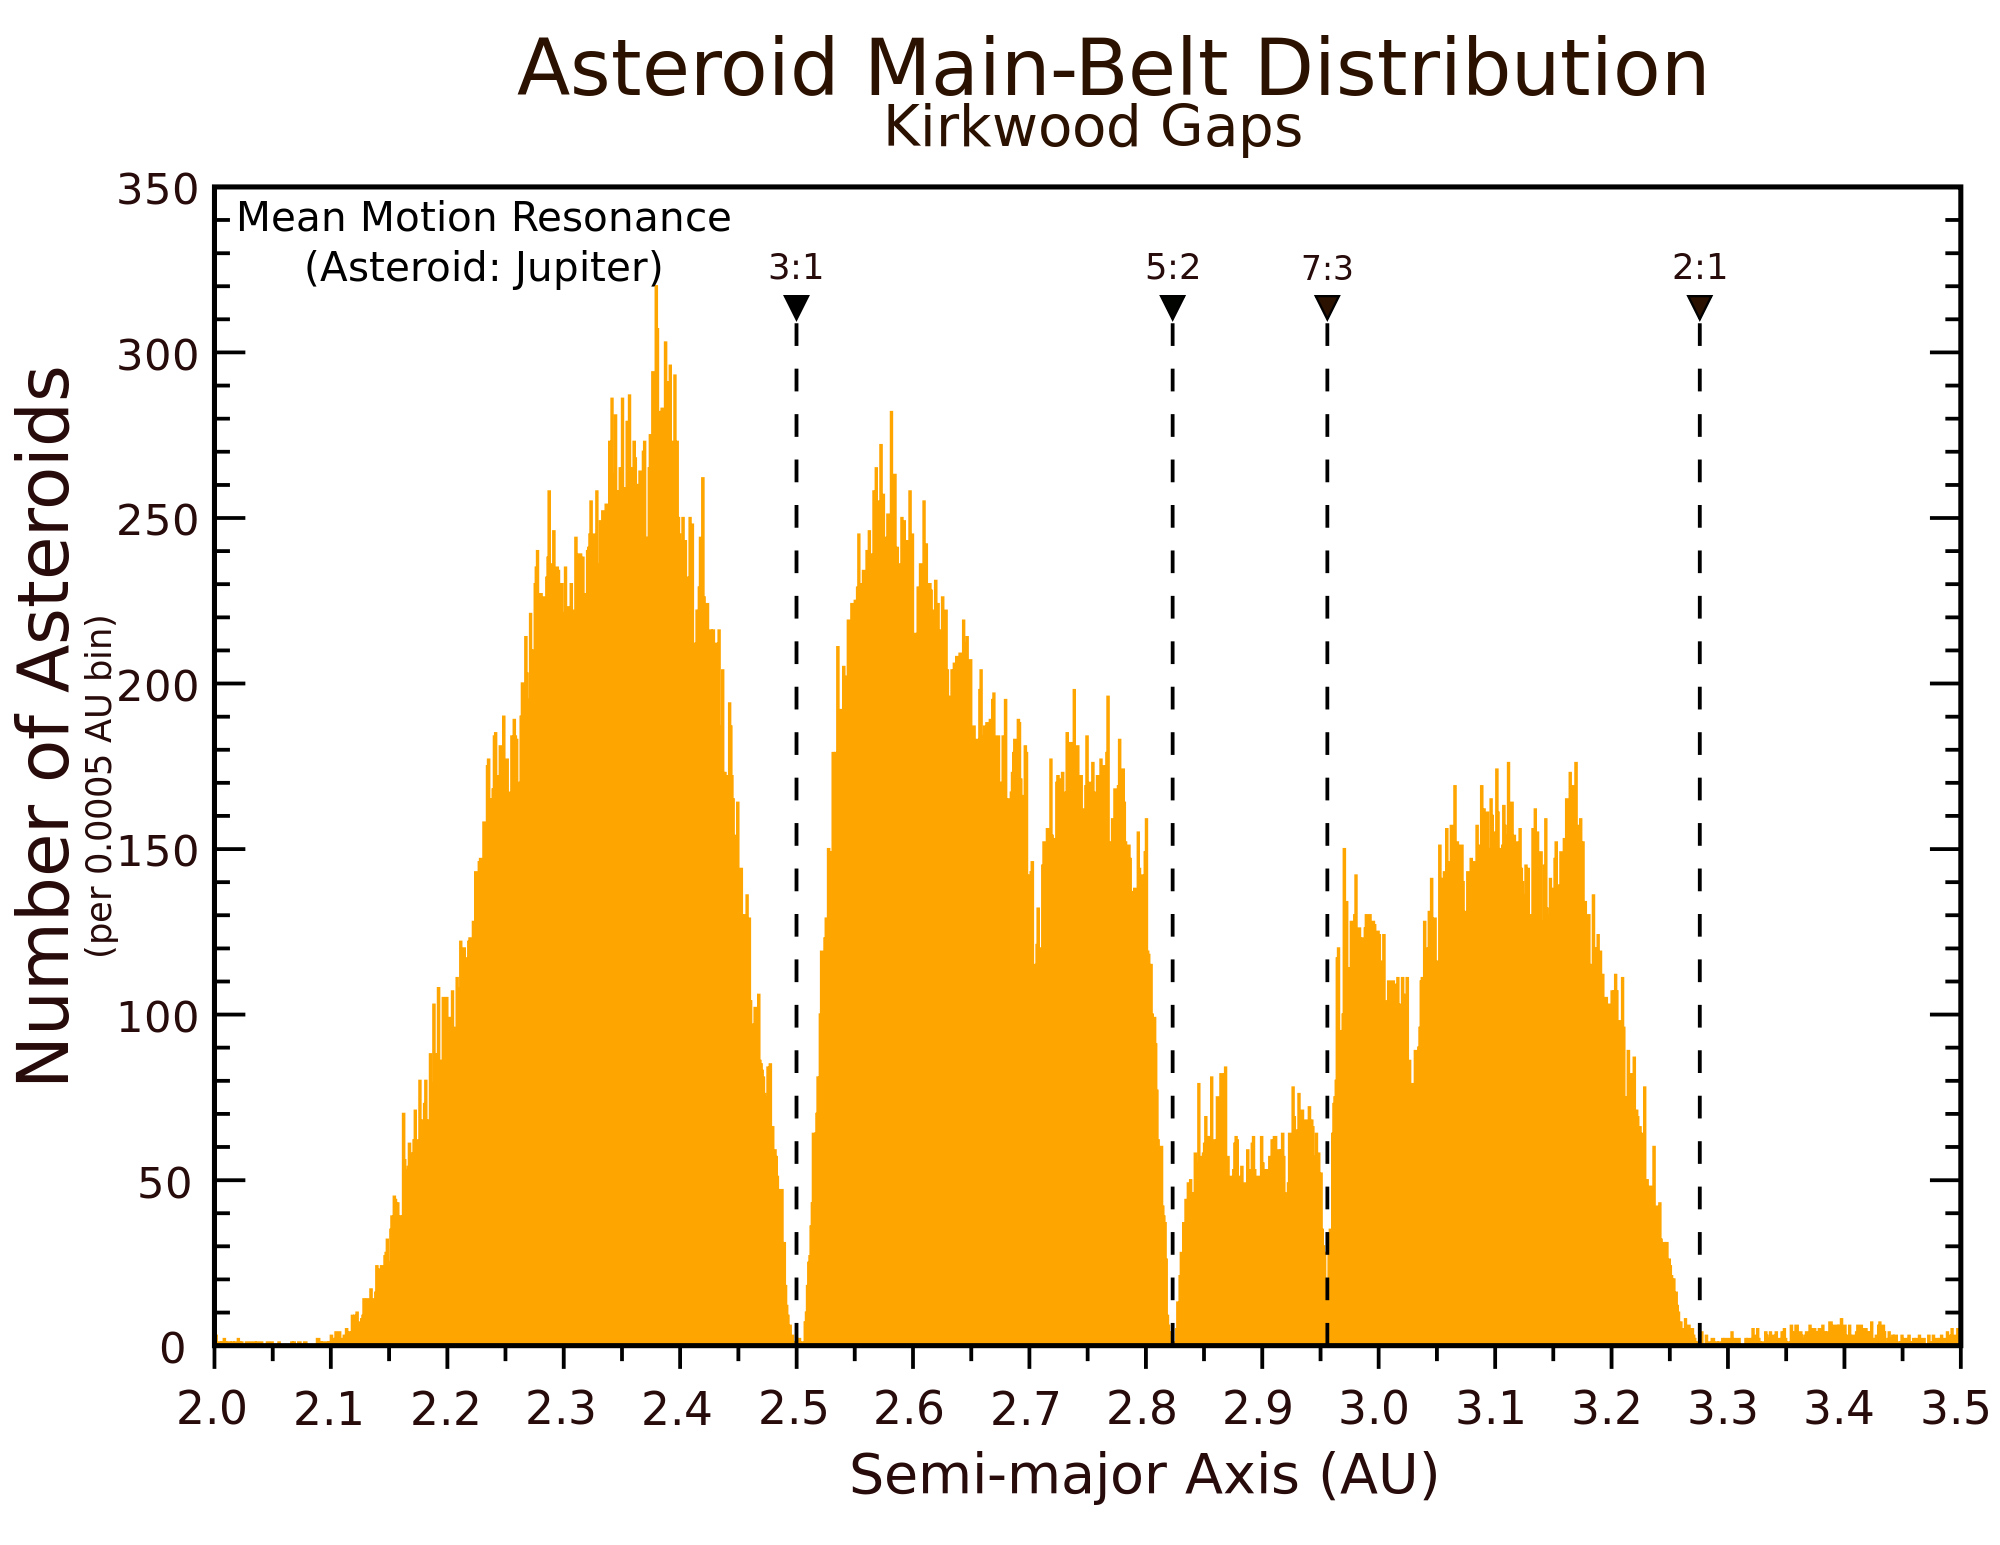
\includegraphics[scale=0.075]{distribution.png}
			
			\small Рисунок 2 --- Пример распределения
		\end{center}
	\end{minipage}
	\end{center}

\end{frame}

% ======== Slide 4 =========

\begin{frame}
\frametitle{Пример таблицы}
	\begin{center}
		\begin{center}
		Таблица 1 --- Название таблицы
		\end{center}
		\small
		\begin{tabularx}{\textwidth}{|X|X|X|X|X|}
			\hline 
			\multirow{2}{*}{Головка} 
			& \multicolumn{2}{c|}{Графа 1} & \multicolumn{2}{c|}{Графа 2} \\
			\cline{2-5}
  			& Подграфа 1 & Подграфа 2 & Подграфа 3 & Подграфа 4 \\ 
			\hline
  			&   &   &   &  \\ 
			\hline
  			&   &   &   &  \\ 
			\hline 
		\end{tabularx}
	\end{center}
\end{frame}

% ======== Slide 5 =========

\begin{frame}
\frametitle{Формулы}
	\label{r1}
	\begin{equation}
	\left\{
  		\begin{array}{rl}
    	\dot x = & \sigma (y-x), \\
    	\dot y = & x (r - z) - y, \\
    	\dot z = & xy - bz.
  	\end{array} \right.
	\end{equation}
	\begin{eqnarray}
	l \quad I
	\end{eqnarray}
\end{frame}


% ======== Slide n =========

\begin{frame}
\frametitle{Публикации (при наличии)}
	\vspace{0.5cm}
	\begin{enumerate}
		\item Публикация 1
		\item Публикация 2
		\item Публикация 3
	\end{enumerate}
	\vspace*{10cm}
\end{frame}
